

\section{Multivariate eda}

Graphical exploration of data is essential.   There are a wide range of techniques for use with multivariate data, this week we examine some of the more common ones.   The aim of this week is to introduce you to some of these techniques, and provide pointers for more advanced ones.   You should save the code you use to generate these graphs in a short script file for future reference!


\section{A correlation paradox}

Here's the correlation paradox we referred to.   Can you explain what's going on here?

\begin{Schunk}
\begin{Sinput}
> u <- rnorm(100)
> v <- rnorm(100)
> w <- rnorm(100)
> x <- u + v
> y <- u + w
> z <- v - w
> X <- cbind(x, y, z)
> cor(X)
> pairs(X)
\end{Sinput}
\end{Schunk}


\section{Key eda techniques}

First, we need to load some data and obtain the most important summary statistics.   We will load data on USArrests as well as irises.   As you go through the lab, if appropriate do try to produce graphs for the other dataset.

\begin{Schunk}
\begin{Sinput}
> data(USArrests)
> `?`(USArrests)
> cov(USArrests)
> cor(USArrests)
> colMeans(USArrests)
> data(iris)
> `?`(iris)
\end{Sinput}
\end{Schunk}

There are then a few ways of producing the ``standard'' pairwise scatterplots.

\begin{Schunk}
\begin{Sinput}
> pairs(USArrests)
> library(lattice)
> splom(USArrests)
\end{Sinput}
\end{Schunk}


As well as examining the relationships between variables, we may be interested in the relationship between individuals.

\begin{Schunk}
\begin{Sinput}
> heatmap(as.matrix(USArrests))
> stars(USArrests, col.segments = c("red", "green", "blue", "pink"), 
+     draw.segments = TRUE, full = FALSE)
> require(MASS)
> parcoord(iris[, -5], col = as.numeric(iris[, 5]))
> source("andrews.R")
> andrews.curves(iris[, -5], cls = iris[, 5])
\end{Sinput}
\end{Schunk}

You can see for example that \texttt{parcoord} and \texttt{andrews.curves} take a data matrix as the first argument (in this case we specify the first four columns of the iris data), and a grouping factor as the second argument (with slightly different syntax).


\section{Interactive Graphics}

You've been given a short piece of code in the portal which helps draw 3d scatterplots on the \texttt{rgl} device.   If you put this code in your working directory and ``source'' it, you should be able to create a simple dynamic 3d scatterplot.   Check out \texttt{?rgl} if you want any help on the rgl device, in particular to see how you might go about saving an image!

\begin{Schunk}
\begin{Sinput}
> source("rglellipsoid.R")
> scatter3d(iris$Sepal.Length, iris$Sepal.Width, iris$Petal.Width, 
+     ellipsoid = TRUE, surface = FALSE, groups = as.factor(iris$Species))
\end{Sinput}
\end{Schunk}


\section{Simulating multivariate normal data and linear combinations}

First, load the \texttt{MASS} library which contains a function \texttt{mvrnorm} which simulates multivariate normal data.   The first argument to \texttt{mvrnorm} is $n$, the number of variate rows to generate, the second argument is the mean vector to use.   Here you see that we want to generate three observations, each with mean zero.   Finally, we need to specify the covariance matrix, we have done this on the previous line and stored the results in \texttt{covmat}.


\begin{Schunk}
\begin{Sinput}
> library(MASS)
> covmat <- matrix(c(1, 0.7, 0.7, 0.7, 1, 0.7, 0.7, 0.7, 1), 3, 
+     3)
> X <- mvrnorm(1000, c(0, 0, 0), covmat)
\end{Sinput}
\end{Schunk}


Having simulated some data (stored in the matrix \texttt{X}), we are going to check the univariate normality of each margin.   The code below produces histograms and plots for the second column, you should check all three!

\begin{Schunk}
\begin{Sinput}
> hist(X[, 2])
> qqnorm(X[, 2])
> qqline(X[, 2], col = "red")
\end{Sinput}
\end{Schunk}
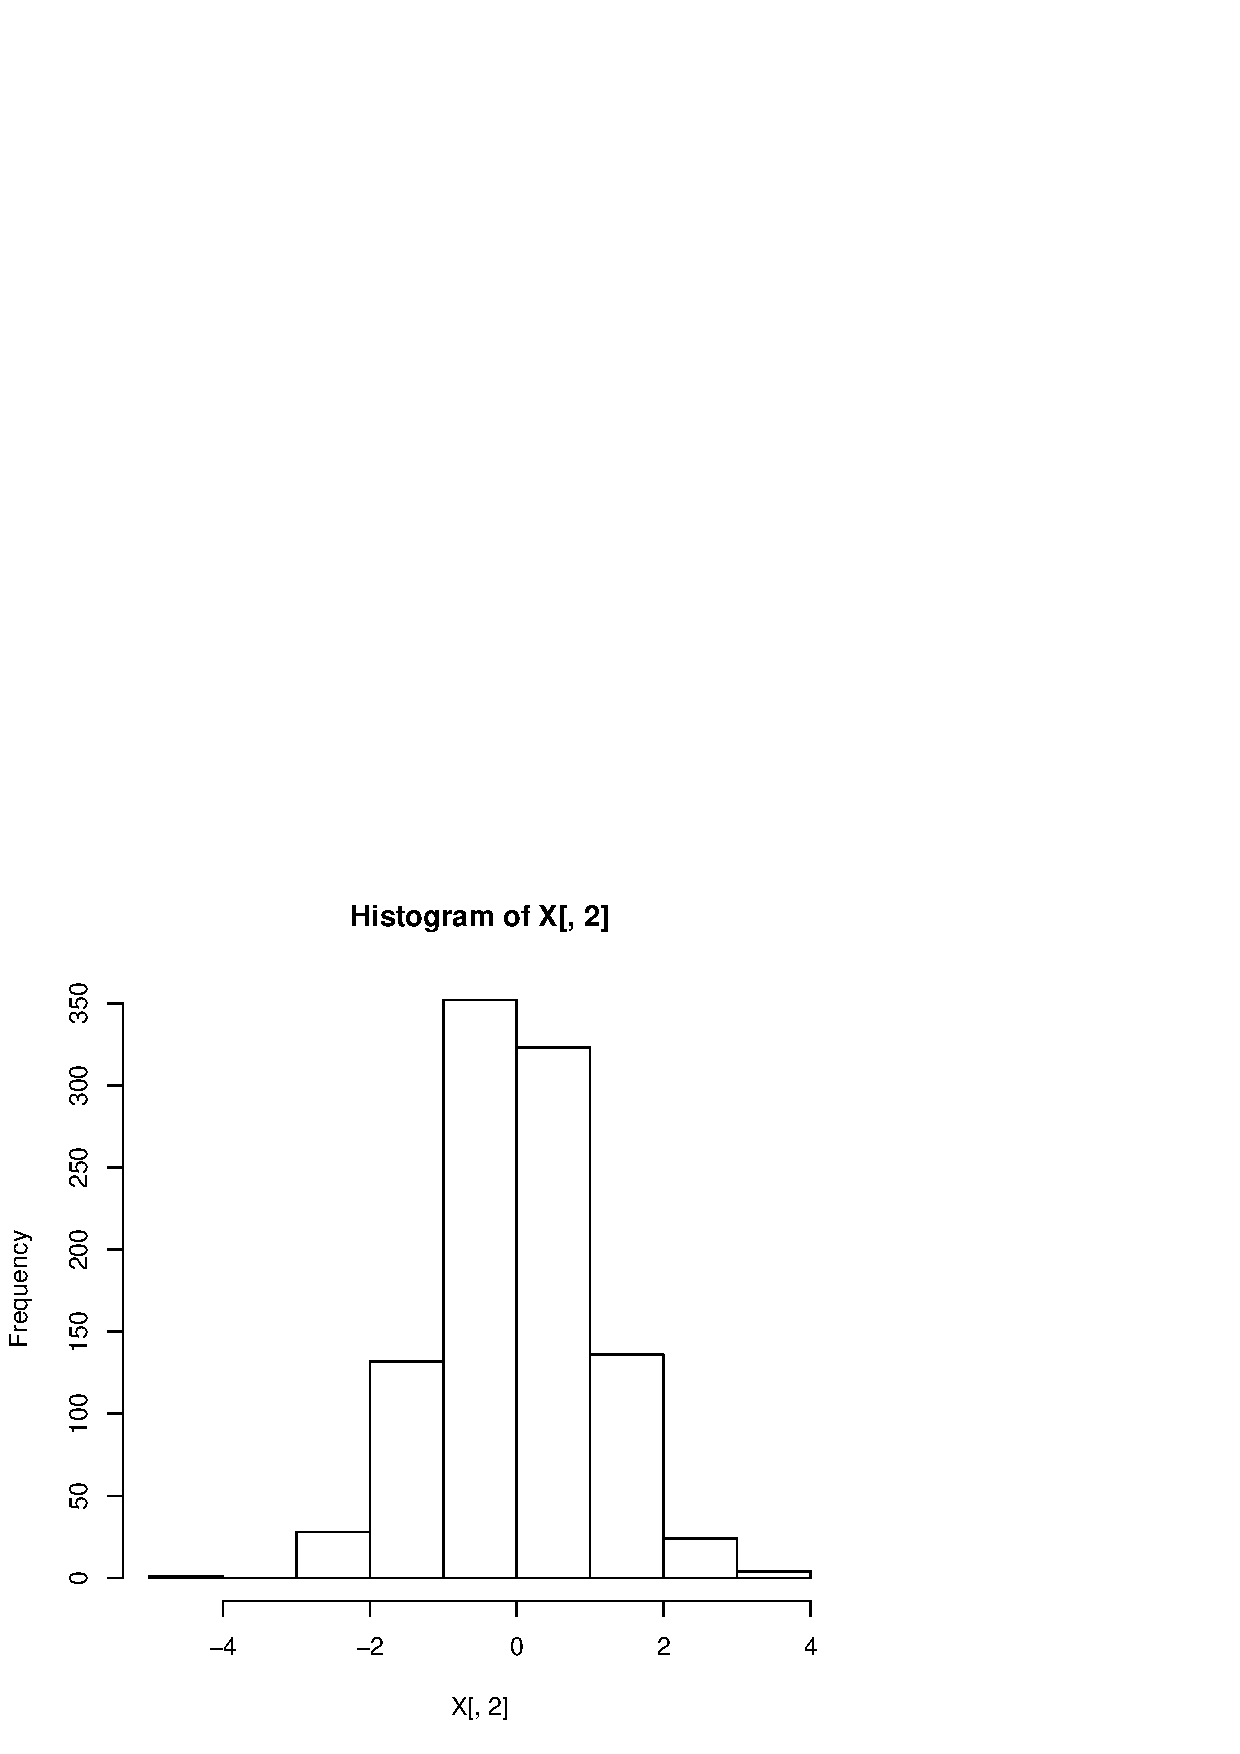
\includegraphics{week1-uvnorm}

Finally, to start thinking about linear combinations, try generating a few linear combinations e.g. $z_{i} = 2x_{i1}+0.2x_{i2}+0.15x_{i3}$ for all $i = 1, \ldots, n$.

\begin{Schunk}
\begin{Sinput}
> Z <- 2 * X[, 1] + 0.2 * X[, 2] + 0.15 * X[, 3]
> hist(Z)
\end{Sinput}
\end{Schunk}

Try different values for the coefficients (i.e replace $2, 0.2 and 0.15$ with other values) and see whether $\boldsymbol{z}$ can be considered to be univariate normal.


\section{On your own}

Load the following libraries, and check out the following functions and data files:   

\begin{itemize}
\item Libraries: \texttt{library(gclus)}, \texttt{library(Flury)}
\item Functions: \texttt{?cpairs}, \texttt{?cparcoord} 
\item Data: \texttt{data(wines)}, \texttt{data(turtles)} and \texttt{data(flea.beetles)} (in other words, load the data and look at the helpfiles in the same way you check the helpfile for a function)
\end{itemize}



Do also check out the correlation demo:

\begin{verbatim}
library(TeachingDemos)
run.cor.examp()
\end{verbatim}








